\subsection{Decision Tree Algorithm}

A binary decision tree is a hierarchical structure that takes input data at its root and propagates it to one of many leaves. Each \emph{leaf} of the tree represents a class designation. To reach a leaf, the features of the data are utilized at \emph{nodes} to make a binary decision: to proceed down the left or right \emph{branch} of the tree? To answer this question, the node also carries a \emph{threshold} that the attribute of the test data is compared against. If the test attribute is less than the threshold, we proceed down the left branch. Otherwise, the right. 

This decision tree structure needs to be generated before it can be used with test data. To train a decision tree that appropriately classifies our test data according to the features we generated, we employ a recursive function. The function signature is
%
\begin{equation*}
  \mathtt{tree = trainDecisionTree(set)}
\end{equation*}

Where \code{set} is the training set, which is a MATLAB structure that contains the raw data (unused), class labels, and generated features. \code{tree} is the returned structure that can be used during testing. It is essentially a nested structure that contains two types of elements: nodes and leaves. At each node of the tree, an attribute and threshold are specified. If a test sample's feature at that particular attribute is less than the threshold, the sample is passed down the left branch of the node. Similarly, if the sample's feature is greater than the threshold, it goes through the right branch. This is repeated until we reach a leaf node, which specifies a class membership. 

The decision tree algorithm has a few major steps, and proceeds by evaluating a metric called \emph{information gain} at various configurations. For now, suffice it to say that information gain is a scalar that represents the improvement in prediction as we narrow down the set (by growing the tree) to find appropriate leaves.
%
\begin{enumerate}
\item Check stopping conditions, which generate leaves.
%
  \begin{itemize}
  \item If there are no more features to split on, return a leaf with the class mode of the set. 
  \item The set is smaller than \code{minLeaf}, which is a tuning parameter that is meant to reduce overfitting of the training data. If this condition is met, return a leaf with the class mode of the set.
  \item If all samples in the set belong to the same class, return a leaf with the class.
  \item If no feature yields an improvement to the information gain (discussed below), then return a leaf with the class mode of the set. Note that this condition is only evaluated after step 2. 
  \end{itemize}
\item Iterate over each feature. Sort the set along the current feature. We utilize a threshold that splits the set between adjacent feature values. Because the information gain across thresholds is convex on the whole (see Fig. \ref{fig:IG}), we use a line search that approximates the highest information gain for each threshold. 

  Let \code{attributeBest} and \code{indBest} be the feature and index that yield the highest information gain. Since the set is sorted, we can simply split the set at the index given by \code{indBest} for the recursion.
\item Recur over the subsets given by \code{indBest} to find the next attribute that yields the highest information gain. Note that we exclude the attribute we chose in this execution of \code{trainDecisionTree(.)}.
\end{enumerate}

This can be expressed in psuedocode as

\begin{algorithm}[H]
\DontPrintSemicolon
\KwData{$set$ of training samples with class labels ($set{2}$) and features ($set{1}$).}
\KwResult{$tree$, a structure containing nodes and leaves.}
\Begin{
  

  $V \longleftarrow U$\;
  $S \longleftarrow \emptyset$\;
  \For{$x\in X$}{
    $NbSuccInS(x) \longleftarrow 0$\;
    $NbPredInMin(x) \longleftarrow 0$\;
    $NbPredNotInMin(x) \longleftarrow |ImPred(x)|$\;
  }
  \For{$x \in X$}{
    \If{$NbPredInMin(x) = 0$ {\bf and} $NbPredNotInMin(x) = 0$}{
      $AppendToMin(x)$}
  }
  \While{$S \neq \emptyset$}{\label{InRes1}
    remove $x$ from the list of $T$ of maximal index\;\label{InResR}
    \While{$|S \cap ImSucc(x)| \neq |S|$}{
      \For{$ y \in S-ImSucc(x)$}{
        \{ remove from $V$ all the arcs $zy$ : \}\;
        \For{$z \in ImPred(y) \cap Min$}{
          remove the arc $zy$ from $V$\;
          $NbSuccInS(z) \longleftarrow NbSuccInS(z) - 1$\;
          move $z$ in $T$ to the list preceding its present list\;
          \{i.e. If $z \in T[k]$, move $z$ from $T[k]$ to
          $T[k-1]$\}\;
        }
        $NbPredInMin(y) \longleftarrow 0$\;
        $NbPredNotInMin(y) \longleftarrow 0$\;
        $S \longleftarrow S - \{y\}$\;
        $AppendToMin(y)$\;
      }
    }
    $RemoveFromMin(x)$\;
  }
}
\caption{Train Decision Tree\label{alg:dt}}
\end{algorithm}

\subsubsection{Information Gain and Entropy}

%
\begin{figure}[H]
  \centering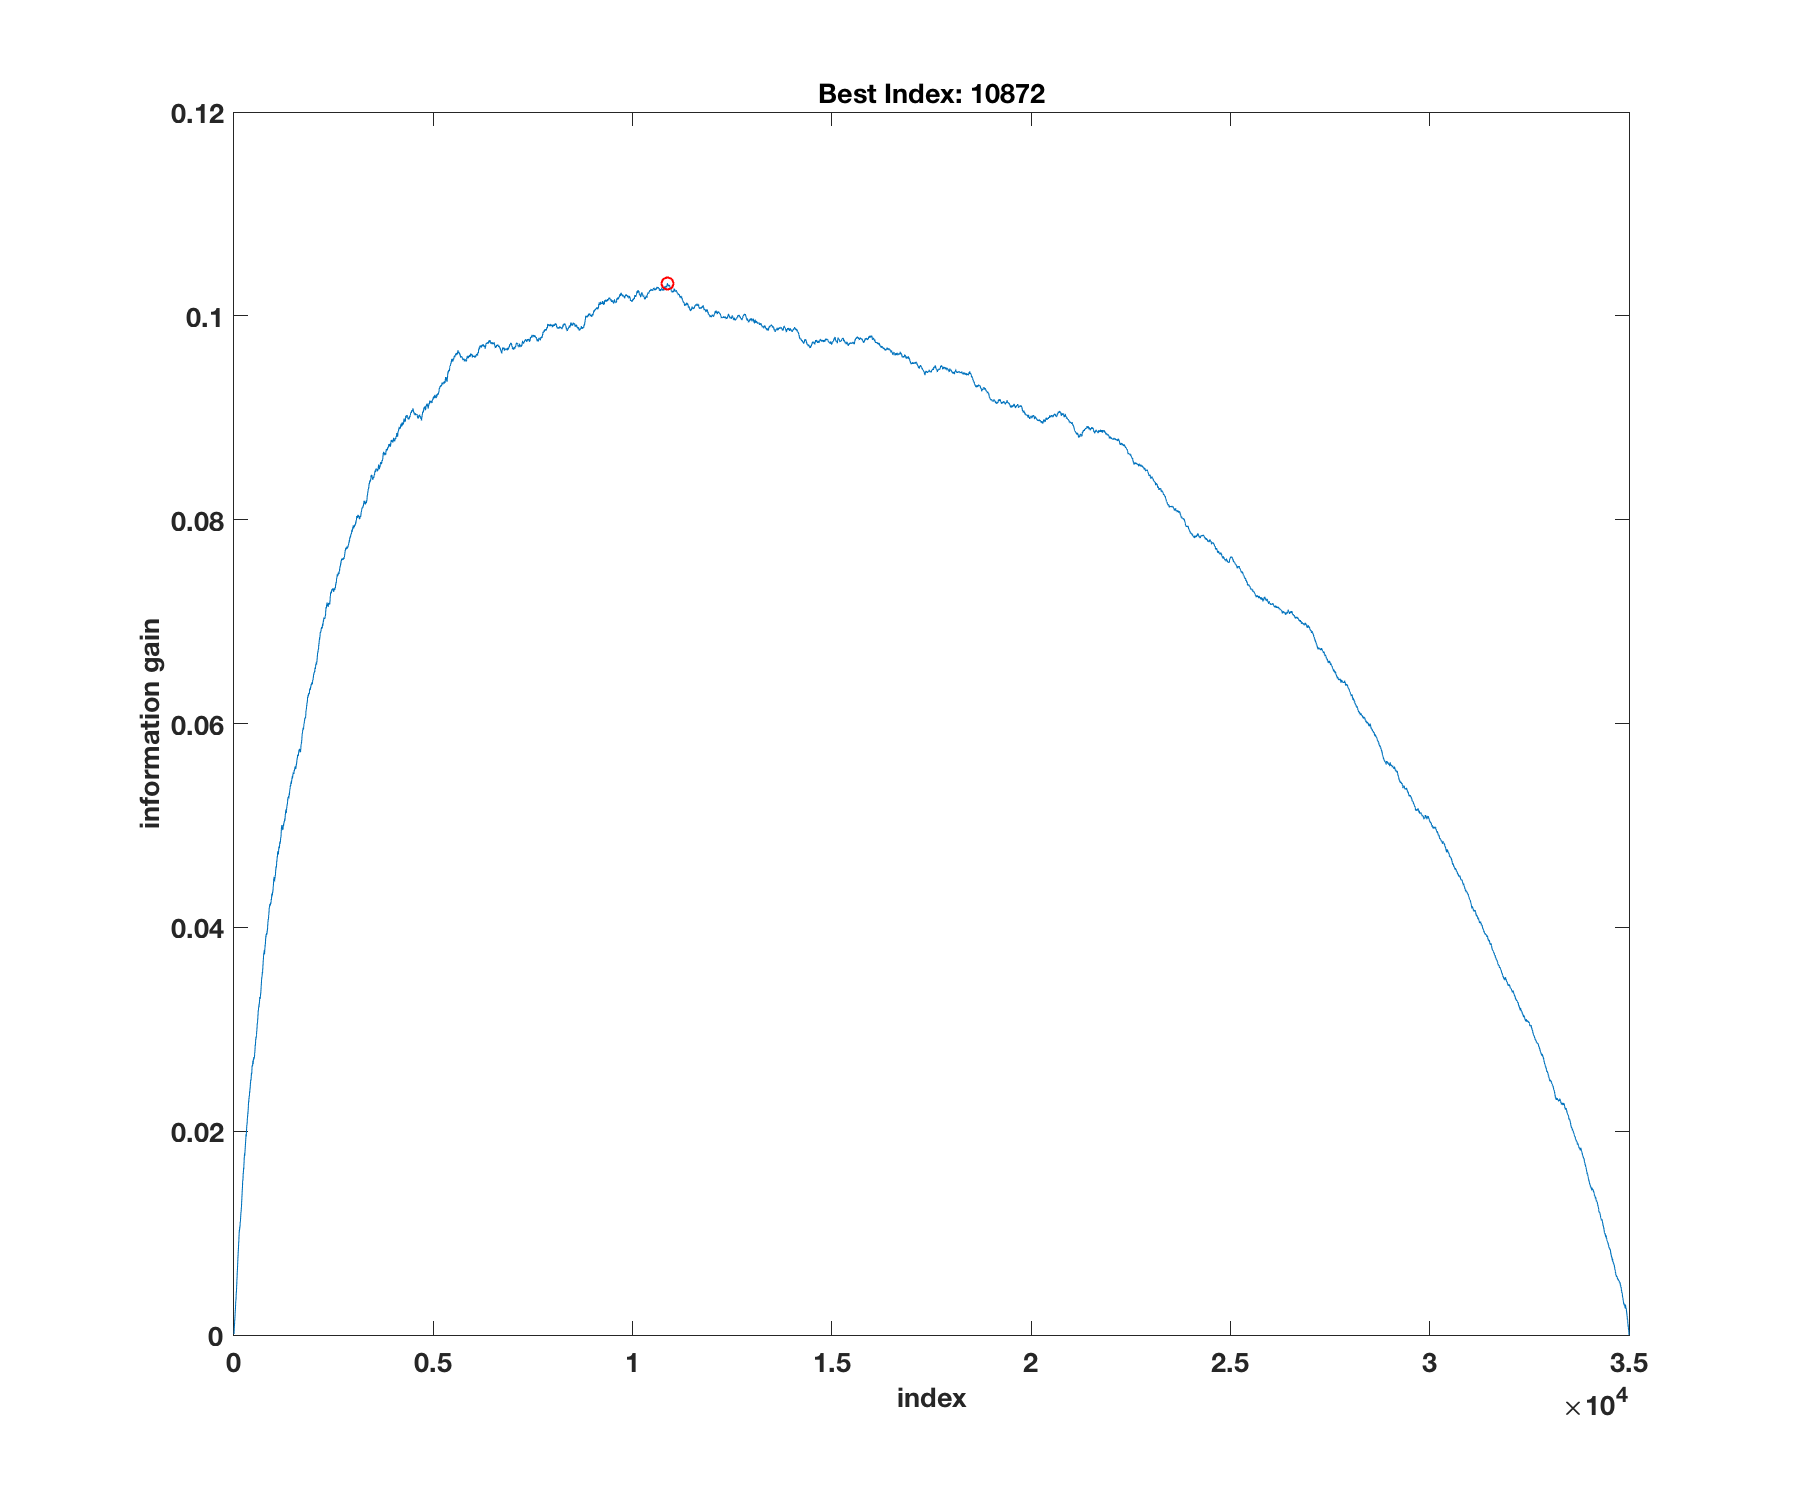
\includegraphics[width=0.6\columnwidth]{images/IG}
  \caption{Information Gain across all possible thresholds.}
  \label{fig:IG}
\end{figure}

